\chapter{Contributo dell'utente}

Come è stato già discusso, nell'ambito della raccolta dei dati il contributo dell'utente
è essenziale. Infatti, è bene che quest'ultimo sia veritiero e che venga fornito per
il maggior numero di registrazioni possibile. Per agevolare l'utente nel dare il contributo
è stato necessario creare un'interazione semplice e che non richiedesse procedure troppo 
sofisticate.\\
Dato che l'informazione che deve essere fornita dall'utente è una etichetta che classifichi
il tipo di parcheggio appena effettuato, è stato deciso di mostrare una notifica di sistema
che proponesse questa scelta. Questa notifica viene chiaramente manifestata dal sistema
sotto forma di notifica locale di GeneroCity e da modo di selezionare il tipo di parcheggio
effettuato (Figura~\ref{fig:flow_diagram_presentazione_notifica}).
\begin{figure}
    \centering
    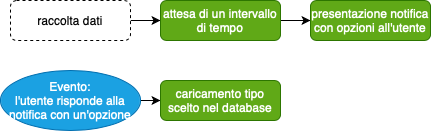
\includegraphics[width=10cm]{images/flow_diagram_presentazione_notifica.png}
    \caption{Diagramma di flusso della presentazione della notifica.}
    \label{fig:flow_diagram_presentazione_notifica}
\end{figure}

\section{Notifica mostrata}

Su piattaforma iOS, è stata scelta la notifica di tipo \emph{Actionable Notification}.
Le notifiche di questa tipologia permettono di aggiungere, oltre al testo, un gruppo 
di pulsanti, corrispondenti a delle azioni. Questa è risultata una soluzione ottima per 
il nostro scopo. \'E stato potuto aggiungere del testo che chiedesse "In che modo hai
parcheggiato?" e allegare dei pulsanti con le opzioni "A spina", "Parallelo", "A pettine".
In questo modo, all'utente resta solo da rispondere alla notifica selezionando una 
opzione tra quelle disponibili (Figura~\ref{fig:presentazione_notifica}).

\subsection{Registrazione della notifica}

Per creare la nuova notifica, la prima cosa che è stato necessario fare è stata registrarla
nel sistema, attraverso l'app. Dato che si tratta di una \emph{Actionable Notification},
è stata registrata una \emph{UNNotificationCategory} e delle \emph{UNNotificationAction}
legate ad essa. Queste classi provengono tutte dalla libreria \emph{UserNotifications}\footnote{
\emph{UserNotifications} page on Apple's website: 
\href{https://developer.apple.com/documentation/usernotifications}{\underline{link to the page.}}}. 
La categoria è necessaria per distinguere una \emph{Actionable Notification}
di un tipo da una di un altro. Quindi, è stata creata una nuova categoria chiamata 
\emph{PARKTYPE}, utilizzata esclusivamente per questa notifica. A questa categoria sono 
state legate le varie azioni, che corrispondono ai tipi di parcheggio. Anche esse sono
dotate di un identificatore che è utilizzato al momento della ricezione, per distinguerle
tra tutte le azioni che l'app può ricevere.
\begin{wrapfigure}{r}{5.5cm}
    \caption{Schermata di GeneroCity con la notifica esposta.}
    \label{fig:presentazione_notifica}
    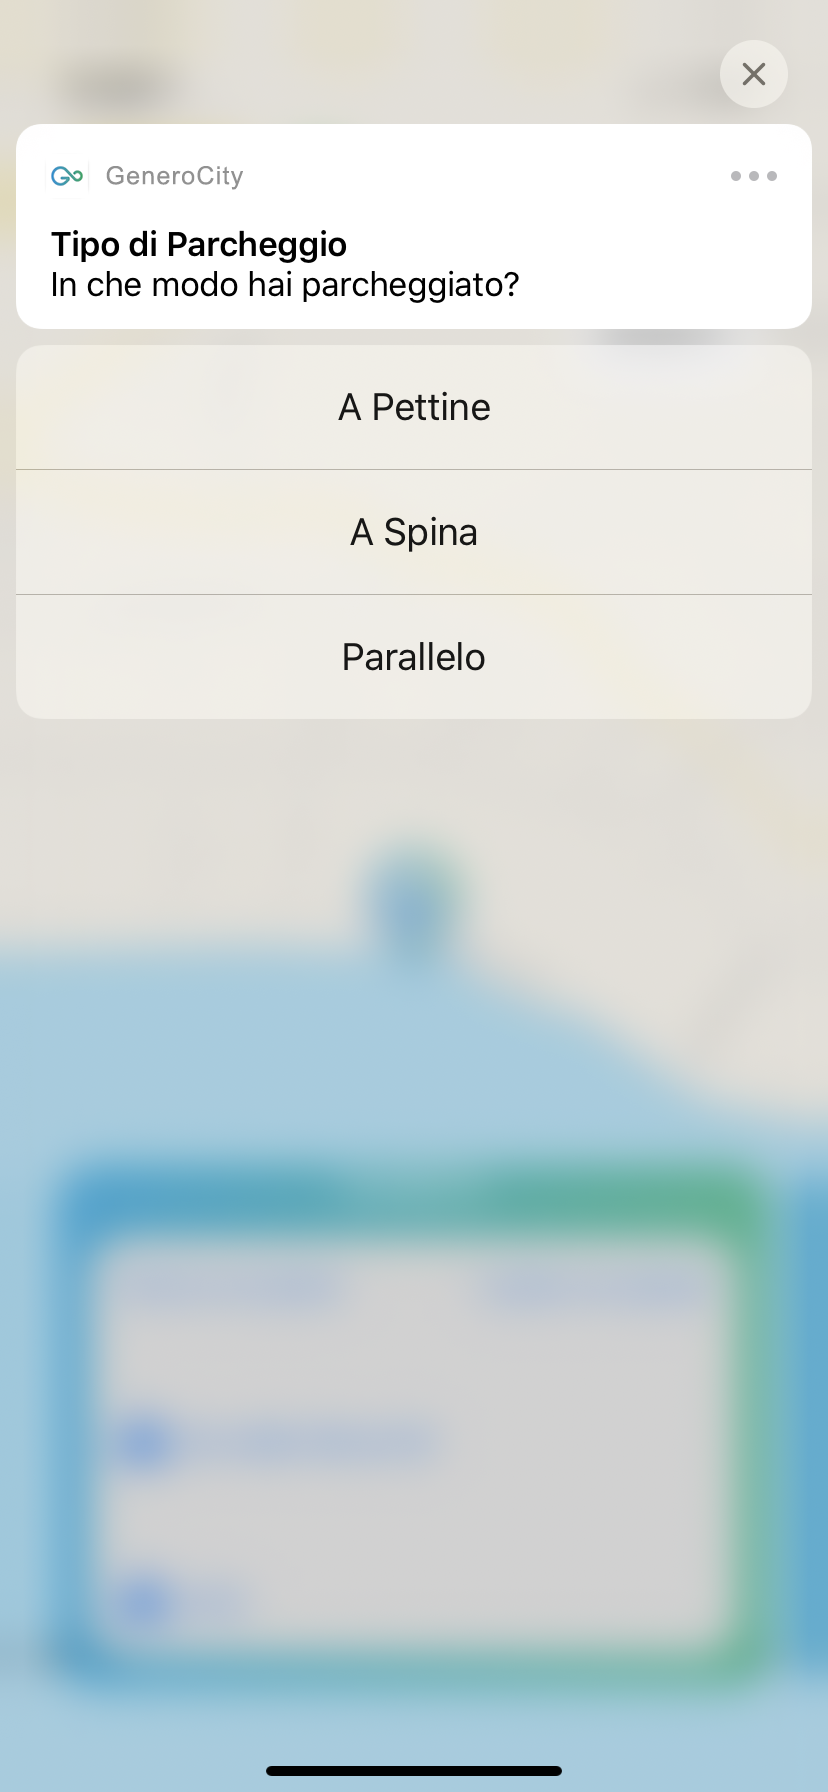
\includegraphics[width=6cm]{images/presentazione_notifica.png}
    \end{wrapfigure} 


\subsection{Esposizione della notifica}

Ogni volta che una nuova registrazione termina, viene creata e mostrata una nuova notifica
con categoria \emph{PARKTYPE}. Per fare ciò, viene creato un
\emph{UNTimeIntervalNotificationTrigger} con un ritardo di 5 secondi. Questo significa che
la notifica verrà effettivamente mostrata all'utente 5 secondi dopo che GeneroCity abbia
rilevato il parcheggio effettuato dall'utente. In questo modo, esso può rispondere alla
notifica quando effettivamente è a conoscenza del tipo di parcheggio appena fatto e
inoltre si è sicuri che non sia più alla guida e quindi non corra rischi perdendo l'
attenzione. % TODO: maybe link here paper "Driver Distraction from Dashboard and Wearable Interfaces"

\section{Etichetta selezionata dall'utente}

Nel momento in cui l'utente riceve la notifica, esso può rispondere scegliendo un'opzione
\cite{options_notification},
oppure ignorarla completamente. Nel caso in cui la notifica viene ignorata, semplicemente 
non accade nulla, ovvero, l'etichetta del tipo di parcheggio non viene caricata sul
database. Invece, in caso contrario, è necessario aggiornare il valore nel database per 
legare l'etichetta appena ottenuta attraverso l'utente, al relativo parcheggio.

\subsection{Ricezione della risposta}

Attraverso il \emph{UNUserNotificationCenterDelegate}, si possono registrare callback 
da eseguire in seguito ad alcuni eventi generati dal sistema, che riguardano le notifiche.
Uno di questi eventi è la ricezione di una risposta. Questa callback viene invocata quando
l'utente clicca su un pulsante azione di una qualsiasi notifica legata all'app.
Questo significa che è compito dello sviluppatore individuare quale azione è stata eseguita
dall'utente, all'interno della callback. Ciò viene fatto attraverso gli identificatori
delle \emph{UNNotificationAction}. Una volta che è stata identificata l'azione scelta,
è possibile capire qual'è il tipo di parcheggio effettuato dall'utente e salvarlo
all'interno dell'oggetto \emph{Car}. Per terminare, viene effettuata una chiamata all'
API del backend, che aggiorni i dati del parcheggio relativo all'auto corrente
nel database.


